\section{Analysis}
\label{sec:analysis}

The experiments in Section~\ref{sec:results} present a consistent picture:
the model learns a genuine correction to $\rho_0$ at fine tree levels
(10--14) but cannot improve on the promolecular density at coarse levels
(1--9). Since the coarse levels determine SCF convergence, the fine-level
improvement has no effect on iteration count. This section explains why.

MADNESS solves the Kohn--Sham equations~\cite{kohn1965self} through a
multi-protocol SCF strategy~\cite{harrison2016madness}. The first
protocol operates at a coarse truncation threshold
($\epsilon = 10^{-4}$), which resolves only tree levels 1 through
approximately 9. At this threshold, the adaptive tree discards all
structure below the coarse truncation scale: wavelet coefficients at
levels 10--14 fall below $\epsilon$ and are projected away when the Fock
matrix is constructed. The SCF cycle at this coarse protocol determines
the number of iterations required and the electronic state reached. Once
the coarse protocol converges, subsequent protocols inherit the
converged coarse density and refine it by adding spatial detail at
progressively finer levels. These later protocols do not revisit the
coarse-level convergence path. They begin from a density that is already
self-consistent at the coarse scale and simply resolve additional spatial
structure (Figure~\ref{fig:tree_schematic}).

\begin{figure}[htbp]
  \centering
  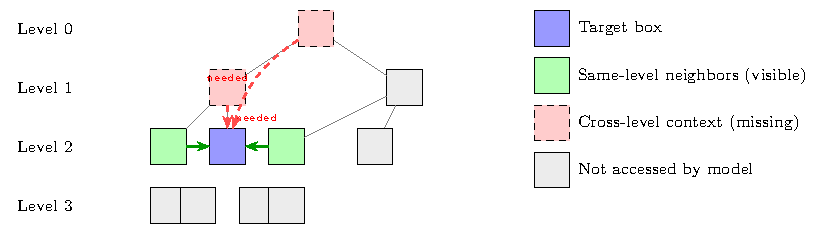
\includegraphics[width=\columnwidth]{figures/fig4_tree_schematic.pdf}
  \caption{Receptive field limitation of the halo-neighbor architecture. The model at a target node (blue) sees only same-level face-adjacent neighbors (green). Cross-level context from parent and root nodes (red, dashed) is needed to capture the global electronic structure that determines the density correction at coarse levels.}
  \label{fig:tree_schematic}
\end{figure}

This multi-protocol structure explains the SCF test results directly.
The level-clamped predictor improves on $\rho_0$ only at levels 10--14.
When MADNESS compresses the initial guess to the first-protocol
threshold, these improvements vanish. The coarse-level density seen by
the first SCF protocol is identical whether the initial guess is
$\rho_0$ or the ML-corrected density. The iteration counts match because
the two initial guesses are, at the resolution that matters,
indistinguishable.

The question then becomes: why does the model fail at coarse levels?
The answer lies in what the input features encode and what the target
correction requires. At any tree level, $\rho_0$ is a smooth
superposition of spherically symmetric atomic densities. $V_\mathrm{nuc}$
is the nuclear Coulomb potential. Both are functions of atomic positions
and species alone. The target correction
$\Delta\rho = \rho_\mathrm{conv} - \rho_0$ encodes
exchange-correlation effects, orbital relaxation, and the redistribution
of electron density due to chemical bonding. These are consequences of
the full many-electron wavefunction. They arise from non-local
electron-electron interactions that the self-consistent field procedure
computes iteratively by solving the Kohn--Sham eigenvalue problem over
the entire molecular domain.

At fine levels (10--14), the correction $\Delta\rho$ is spatially
localized near nuclei and varies smoothly as a function of the local
atomic environment. Same-level halo neighbors provide enough context for
the model to interpolate this correction from training data. At coarse
levels, $\Delta\rho$ reflects global electronic structure: how orbitals
delocalize across the molecule, how exchange-correlation modifies the
density at scales comparable to bond lengths, and how the occupied
orbital space responds to the full molecular potential. The input
features at a coarse node, consisting of $\rho_0$ and $V_\mathrm{nuc}$
at that node and its six face-adjacent neighbors, do not contain this
information and cannot contain it. The promolecular density and nuclear
potential at a handful of neighboring boxes encode atomic positions and
charges, not the self-consistent electronic response to those charges.

This is not a model capacity problem. The parent feature experiment
(Section~\ref{sec:parent_features}) increased parameters from 3.0M to
4.1M with no change in coarse-level accuracy. It is not a data
problem. Expanding the training set from 15 to 51 molecules improved
fine-level predictions but left coarse-level ratios unchanged at
1.00--1.12$\times$ baseline. It is an input sufficiency problem: the
mapping from $(\rho_0, V_\mathrm{nuc})$ to $\Delta\rho$ at coarse
levels is not a well-defined function of those inputs. Multiple
distinct corrections $\Delta\rho$ can arise from the same local
$\rho_0$ and $V_\mathrm{nuc}$ pattern, because the correction depends
on the global molecular context that the local inputs do not resolve.

Could a different architecture overcome this limit? The parent feature
experiment tested the simplest form of multi-scale context: concatenating
the $\rho_0$ and $V_\mathrm{nuc}$ coefficients from the parent node.
This expanded the receptive field to span two tree levels, but the
additional information was a coarser copy of the same signal. A graph
neural network or attention-based architecture that aggregates
information across the entire tree would have access to every node in
the adaptive representation. However, if the node-level features remain
$\rho_0$ and $V_\mathrm{nuc}$, then global aggregation produces a
summary of the promolecular density and nuclear potential, not of the
self-consistent density. The quantity the model needs to predict, the
electron-electron interaction correction, is precisely what is absent
from these inputs. No aggregation scheme over $\rho_0$ and
$V_\mathrm{nuc}$ can reconstruct $\Delta\rho$ at coarse levels, because
$\Delta\rho$ is not a function of $\rho_0$ and $V_\mathrm{nuc}$ alone.
It depends on the solution of the Kohn--Sham equations, which is the
output of the SCF procedure, not a property of the input potential.

This is the fundamental limit. A local ML model that takes the
promolecular density and nuclear potential as input and produces a
density correction as output is attempting to bypass the SCF iteration
by learning its fixed point from input data that does not determine
that fixed point. The model succeeds at fine levels because there the
fixed-point correction happens to be a smooth, spatially localized
function that correlates with the local atomic environment. It fails
at coarse levels because there the correction is a global property of
the electronic state. The multi-protocol SCF structure of MADNESS then
ensures that only the coarse-level result affects convergence speed.
The fine-level success, while real, is operationally irrelevant.
